% TODO: maybe add another section about how vectorization actually works in archetypes vs types?

\section{Concurrency Model}
The following concurrency model is of my own design. To the best of my ability I was unable to find a model like the one presented in this paper other than FLECS to a degree. Since our implementations follow similar techniques such as using archetypes and being a dense ECS, our concurrency models seem to overlap slightly but further investigation is needed.

\subsection{Formal definition} \label{section:formal_definition}
In this paper, we define an Entity Component System, short for ECS, to be a tuple $W = (T, A, \delta, \Lambda)$ consisting of:
\begin{enumerate}
    \item A finite set of types $T$
    \item A set of archetypes $A \subseteq \mathcal{P}(T) \cup \emptyset$, where $\mathcal{P}(T)$ denotes the power set of $T$    
    \item Some transition function $\delta : A \times T \rightarrow A$
    \item A set of systems $(\lambda, \lambda_{req}) \in \Lambda$ such that $\lambda : W \rightarrow W$ and $\lambda_{req} \subseteq \mathcal{P}(T)$ representing the types required to initiate $\lambda$
\end{enumerate}

\subsection{Types And Archetypes}
Until now, components were only stored in homogenous vectors which is great for cache locality but it introduces some problems -- namely with composite entities. We define a type $T$ to be the reference to a class of components. Therefore, a homogenous vector contains only components of type $T$.

\subsubsection{The ABC Problem}
% https://ajmmertens.medium.com/building-an-ecs-2-archetypes-and-vectorization-fe21690805f9
The ABC Problem is a problem introduced by the FLECS creator Sander Mertens. It's a problem that demonstrates the effectiveness of Archetypes in component storage and is a good introduction.

Outside of ECS world $W$, we define a set of entites $E$ and $n = |E|$. Suppose $T := \{A,B,C\}$ and for each type $t \in T$, there exists a homogenous vector containing elements of type $t$. If all entities have all the components then:

\begin{figure}[H]
    \begin{lstlisting}[
        language=Java,
        style=colored
    ]
    A components[n];
    B components[n];
    C components[n];
    \end{lstlisting}
    \caption{Homogenous ECS Components}
    \label{code:homogenous_ecs}
\end{figure}

In this ideal world, entity ID can be emulated by the index to all vectors because the property $\forall t \in T : |t| = n$ holds. This ECS is positioned advantageously because the code is vectorizable and we can guarentee all components are contiguous in this design. 

Suppose one of the entities at some index $k$ removes one of its components from component $t$. In such a situation, the defined indexing property is broken because not all vectors are of the same length and it is now impossible to write vectorized code for this ECS.

Sander Mertens uses this setup to prove that an ECS cannot vectorize homogenous components at all. This is done by reviewing all situations in which homogenous components are unable to recover from runtime updates. By the end, he presents an alternative called archetypes and proves that archetypes leads to some form of good vectorizability.

\subsubsection{Archetypes}
Simply put, an archetype is a set of types as defined in section \ref{section:formal_definition}. Archetypes add a layer of abstraction on top of types so to make ECS queries vectorizable. Instead of creating homogenous vectors based on types in $T$, we can create homogenous vectors based on archetypes in $A$. 

\begin{figure}[H]
    \begin{lstlisting}[
        language=Java,
        style=colored
    ]
    // Type {A}
    A a[A_len];
    // Type {A, B}
    A a[AB_len];
    B b[AB_len];
    // Type {A, C}
    A a[AC_len];
    C c[AC_len];
    \end{lstlisting}
    \caption{ECS Components With Archetypes $\{\{A\},\{A,B\},\{A,C\}\}$}
    \label{code:ecs_archetypes}
\end{figure}

Even though in Figure \ref{code:ecs_archetypes} those arrays are independent they do not have to be. In my implementation, for example, all components in an archetype are interleaved in a contiguous array. So essentially the papers archetypes storage looks more similar to Figure \ref{code:homogenous_ecs} than Figure \ref{code:ecs_archetypes}.

\subsection{Representing Archetypes As An Entity Finite-State-Machine}
\label{sec:fsm_arc}
ECS applications are expected to handle operations over entities that can add, modify, or remove components. In the context of archetypes, this means being able to transition an entity between archetypes. 

An example of such a situation is a game. Suppose all entities within the proximity of some point in space gain a tag component saying "buffed", but when they leave the proximity the tag component is removed. These types of state transitions may occur hundreds of times and need to be performant.

\subsubsection{Archetype Graphs}

A finite state machine emerges from using archetypes to organize entities in a specific way. If the addition and removal of components are considered as state transitions, then the following in Figure \ref{fig:graph1} represents existing archetypes during some ECS runtime. We define vertices to be archetypes in $W$ and edges to be component addition or removal transitions to adjacent archetypes.

As an example, suppose we have an ECS with the following properties:
\begin{align}
    T &= \{A,B,C,D\} \\
    A &= \{ \emptyset, [A] , [A,C] ,[B], [A,B], [A,B,C], [B,D], [D]\} \\
    \Lambda &= \emptyset
\end{align}

\begin{figure}[htbp]
    \centering
    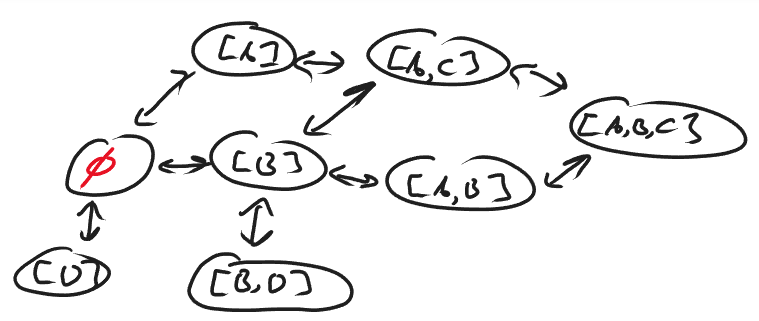
\includegraphics[width=0.5\linewidth]{resources/graph1.png}
    \caption{Example FSM Graph Of Archetypes During Runtime}
    \label{fig:graph1}
\end{figure}

As shown in Figure \ref{fig:graph1}, all graphs contain the empty set $\emptyset$ as a vertex. This is because all entities when initiated contain the the archetype with no components. As components get added to entities over runtime, the entities shift their components to different vertices as their archetype changes, building out the graph.

Archetype graphs display the following properties:

\begin{enumerate}
    \item All existing archetypes must have a path to vertex $\emptyset$.
    \item Components can appear multiple times.
    \item Archetypes can only appear once.
\end{enumerate}

There are a couple interesting things to notice in Figure \ref{fig:graph1}. Notice how there is no transition between state $[B,D]$ and $[D]$. This is because this graph represents a runtime of an ECS and not the complete graph of all possible transitions. 

The component $C$ in Figure \ref{fig:graph1} is special in the regard that it is not adjacent to the $\emptyset$ vertex. This does not mean that it is impossible to create an entity with only $C$ but that the runtime has yet to have that situation occur.

To loop back to the proximity example in section \ref{sec:fsm_arc}, by representing archetypes as runtime state transitions we can now see that large performance gains are achieved via caching. Initially, for the first item in the simulation it will be slow because the edge between those two vertices must be made. Once that edge is made, it is cached and the deletion and transfer of an entity to another archetype drops from $O(N)$ to $O(1)$.

\subsubsection{Opertions On Entity FSM}
The following operations are all thread safe due to the scheduling algorithm explained in section \ref{sec:scheduling}. All implementation details are abstracted away except the operations directly done on the graph. 

\textbf{Entity Creation:} All entities when created start at the $\emptyset$ vertex. All entities that exist here are not queryable. In the papers implementation, the $\emptyset$ vertex is used as a garbage collection tool. All entities waiting for deletion are transitioned to the empty set and cleaned at the end of the tick. 

\textbf{Entity Component Addition: } Aside from the simple transition using an existing edge. When a component addition occurs two operations are completed. Suppose the archetype we are currently in is a set of types $G$ and are attempting to add component $C$. The two operations are the lookup operation and the connection operation.

\begin{enumerate}
    \item If $G \cup \{C\} \not\in A$, then do step 2. Else do step 3.
    \item Create a new archetype $G \cup \{C\} \in A$.
    \item Create the edge $G \leftrightarrow G \cup \{C\}$.
\end{enumerate}

When considering concurrency, data invalidation can occur if the archetype to transition to exists and another thread or system is using that archetype. In such a situation, the papers implemention waits for that part of the graph to be free'd.

\textbf{Entity Component Deletion: } When an entity is marked to have a component deleted. The same algorithm is used in entity component addition. Both addition and deletion use the same transition function $\delta$ of the papers ECS definition.  

\textbf{Entity Deletion: } When an entity is marked for complete deletion, the archetype it was part of must have at least one more entity to exist. If the archetype is empty, it must be removed from the graph. While this property keeps the graph mathematically pretty, there is no reason to programatically remove cached edges as they have a probability to appear again. The memory usage of an empty archetype is inconsequential. 

\subsection{Scheduling Systems}
\label{sec:scheduling}

Due to the nature of ECS architectures following some principles of data-oriented design, ECS architectures have an advantage in concurrency contexts. The following section is about an algorithm designed in this paper to schedule what is parallelizable and what is not parallelizable. This algorithm does not guarentee that all entities will run at the same time, but does guarentee that all entites will have been processed once per tick at some point in time. Such is the nature of concurrency. 

\subsubsection{Syntax Introduction}
For the following algorithms in section \ref{sec:scheduling}:

\textbf{Partial Systems:} A partial system $\lambda'$ is defined as a system the processes a specific set of archetypes, instead of its requirements.

\begin{equation}
    \lambda^\prime := \{a_1,a_2,\ldots,a_n\} \in \mathcal{P}(A) : \lambda[a_1][a_2]\ldots[a_n]
    \label{eq:partial_lambda}
\end{equation}

\textbf{Set Symmetric Difference:} $\Delta$ used in the following algorithms is defined as the symmetric difference: 
$$x_1 \Delta x_2 := (x \cup x_1) \setminus (x \cap x_1)$$

\textbf{Threads:} The total threads allocated for the ECS is also defined as $t$. \\

\subsubsection{Partitioning Algorithm}
\label{alg:part}
The following algorithm presented in the paper is used to determine what systems are parallelizable based on the entity FSM introduced in section \ref{sec:fsm_arc}. 

\begin{enumerate}
    \item Initiate sets $par$ and $seq$ that will contain data of type $\lambda^\prime$.
    \item Initate a vector $v_1$ that will contain tuples $(\lambda \in \Lambda, x \subseteq A)$
    \item For each $\lambda \in \Lambda$, we do the following steps 4-5:
    \item Construct the set x such that $x = \{ \forall a \in A : a \cap \lambda_{req} \not= \emptyset \}$
    \item Push to $v_1$: $(\lambda, x)$
    \item For each $(\lambda, x) \in v_1$, we do the following steps 7-10:
    \item Calculate the set $X_{seq} = \{ \forall (\lambda_1, x_1) \in v_1, : x \cap x_1  \land x \not= x_1 \}$. $X$ contains all archetypes that $\lambda$ cannot do in parallel.
    \item Calculate the set $X_{par} = \{ \forall (\lambda_1, x_1) \in v_1, : x \Delta x_1  \land x \not= x_1 \}$. $X$ contains all archetypes that $\lambda$ can do in parallel.
    \item Push to set $seq$ the value $ \forall x_0,x_1,\ldots,x_n \in X_{seq} : \lambda[x_0][x_1]\ldots[x_n]$
    \item Push to set $par$ the value $ \forall x_0,x_1,\ldots,x_n \in X_{par} : \lambda[x_0][x_1]\ldots[x_n]$
\end{enumerate}

After all the steps above, the sets $seq$ contains all archetypes that cannot be run in parallel and the set $par$ contains all archetypes that can be run in parallel.

Although the algorithm for partitioning in section \ref{alg:part} is $O(N^2)$ where $N$ is the number of archetypes, its unlikely that there will ever enough types of components and lazily loaded archetypes on the graph for it to matter in any circumstance, but it is important to still bring awareness.

% TODO: ACTUALLY DO IT
Depending on the leniency of defining $\lambda_{req}$, its possible to only ever have to do this calculation once. If all systems are defined at compile time and new systems are not allowed to be added during runtime, the computation graph will never change. The implementation in this paper allows new systems to be defined at runtime and only needs to recalculate on new archetype additions to the Entity FSM.

\subsubsection{Example Run}
To show this algorithm in process, the following uses Figure \ref{fig:graph1} as an example to go through. Suppose instead of $\Lambda = \emptyset$:

\begin{equation*}
\Lambda = \begin{cases}
    \lambda_1 &= [A,C] \\
    \lambda_2 &= [B,C] \\ 
    \lambda_3 &= [D]    
\end{cases}
\end{equation*}

Following through with steps 1-4, the vector $v_1$ will contain the following:

$$
v_1 = \left[
\begin{array}{@{}l@{}}
(\lambda_1, \{[A],[A,B],[A,C],[A,B,C]\}) \\
(\lambda_2, \{[B],[A,B],[B,D],[A,C],[A,B,C]\})\\
(\lambda_3, \{[D],[B,D]\})
\end{array}
\right]
$$

Now to step 6, where we calculate for each $(\lambda, x) \in v_1$ the parallel and not parallelizable sets. For brevity I will only show the process for $\lambda_2$ and show the final results of this step for all systems:

To calculate the non-parallelizable set for $\lambda_2$ we do the following:
\begin{align*}
\lambda_2 \cap \lambda_1 &= \{[A,C],[A,B],[A,B,C]\} \\
\lambda_2 \cap \lambda_3 &= \{[B,D]\}    
\end{align*}

To calculate the parallelizable set for $\lambda_2$ we do the following:
\begin{align*}
\lambda_2 \Delta \lambda_1 &= \{[A]\} \\    
\lambda_2 \Delta \lambda_3 &= \{[D]\}    
\end{align*}


\subsubsection{Computation Graphs}
Now with $par$ and $seq$, we are able to generate the computation graph for the systems. We sequentially process all partials in $seq$ first, and then spin up threads for each system. 

\begin{figure}[H]
    \centering
    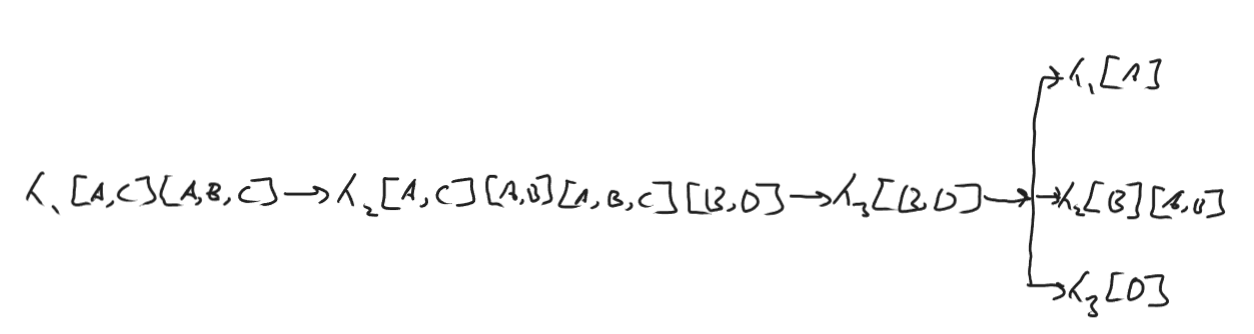
\includegraphics[width=0.5\linewidth]{resources/computation_graph.png}
    \caption{Temp Graph To Replace Later with Latex}
    \label{fig:temp1}
\end{figure}

There is a visual way to understand this algorithm. A BFS can be initiated from all starting types from the given $\lambda_{req}$ to capture the vertices in $v_1$. Then we color each vertex set with unique colors. 

\begin{figure}[H]
    \centering
    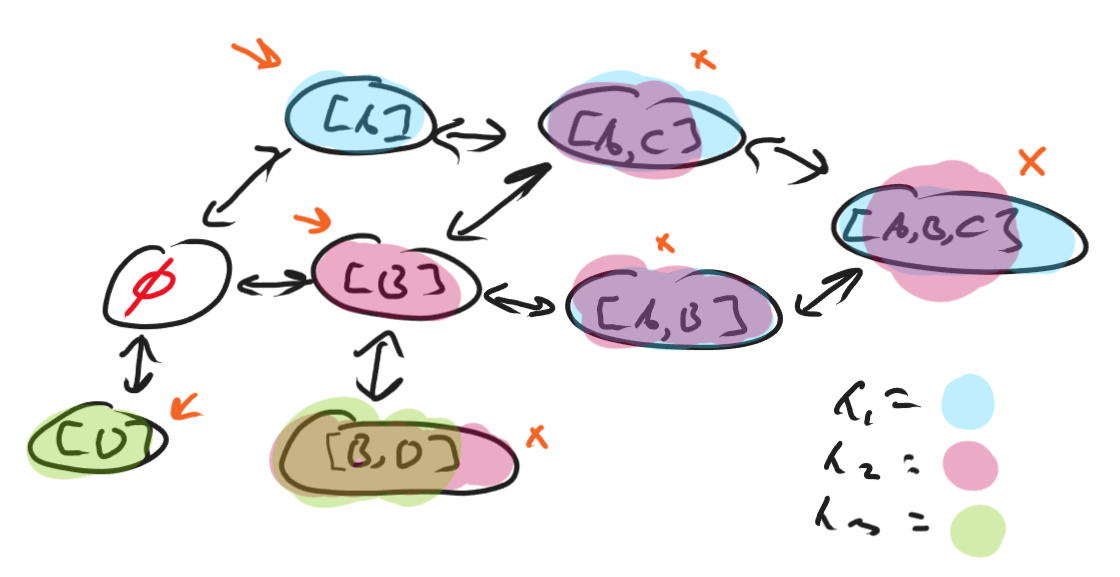
\includegraphics[width=0.5\linewidth]{resources/color_graph.png}
    \caption{Temp Graph To Replace Later with Latex}
    \label{fig:graph2}
\end{figure}

In Figure \ref{fig:graph2}, notice that all nonoverlapping colors are safe to multithread while all overlapped colors ended up in the sequential part of the computation graph.

\subsubsection{Scheduling Systems}
Now to finally scheduling the systems. Because of the hard work done in section \ref{alg:part}, the set $seq$ can just run sequentially so that will be ignored and processed on the main thread. Once those are done, we assign for each partial system $\lambda^\prime \in par$ to the next available thread in the thread pool. 

\subsection{Entity Consolidation}
A key concept omitted thus far is how entities interact with the Entity FSM in concurrent contexts. There are three things in which an entity can do:
\begin{enumerate}
    \item Add a component and transition to a vertex not dependent on other concurrently running systems. 
    \item Add a component and transition to a vertex dependent on other concurrently running systems. 
    \item Move to $\emptyset$.
\end{enumerate}

\subsubsection{$\delta$ Transition To Non-Dependent System}
This case handled by the partitioning algorithm. Each entity, while running in the concurrent context, cannot appear twice in the same concurrent context. Entities can appear multiple times but never more than once while in the concurrent context. This is because archetypes organize entities and archetypes are what defines a partial system. 

\subsubsection{$\delta$ Transition To Dependent System}
% TODO: ACTUALLY DO THIS
This case can be handled in various ways. The easiest way is to add a constraint to $\lambda$ stating that operations such as these are invalid and must be included in the $\lambda_{req}$ set. The method this papers implementation chose is to have a local ledger of conflicting changes stored at the starting vertex. By doing this, we ensure that all concurrent systems finish with the same set of entities they deterministically started out on. Before the end of each tick, the ledgers of all vertices will be wipes and all entities with their accompanying data will be transfered to where they belong.

The ledger is defined as a map between entity ids and a queue of archetypes. If the entity wishes to transition to an archetype that is running concurrently, the entity will push the archetype to the queue. The full algorithm is detailed below:


\textbf{On Component Add:}
\begin{enumerate}
    \item An entity $e$ has requested for it to move from archetype $A$ to archetype $B$.
    \item Check if entity exists in the ledger. If so, go to step 3. Else, skip.
    \item Enqueue to entity $e$ archetype $B$. Done.
    \item Check if archetype $B$ belongs to another concurrent system. If so, go to step 3. Else, skip.
    \item Transition entity $e$'s archetype to $B$. Done.
\end{enumerate}

\textbf{On Archetype Move:}
\begin{enumerate}
    \item For each $a \in A$, do the following steps:
    \item For each $(e, q) \in a$ where $e$ is the entity and $q$ is the queue of types to apply.
    \item While $q$ is not empty, dequeue into $q^\prime$. If empty, Go to step 6.
    \item Transition entity $e$'s archetype to $q^\prime$.
    \item Go to step 2.
    \item Done.
\end{enumerate}

It's important to note that in such scenarios it's not only the new archetype that get's queue'd but the new component as well. The user must be able to dynamically construct and use these components while they are on the ledger unmoved. My implementation handles this.

\subsubsection{$\delta$ Transition To $\emptyset$}
This case is the deletion case and is handled using the same ledger in case 2. We push onto the ledger $(e \in E, \emptyset)$. Before the end of the tick, we iterate and clean out all entities that are supposed to transition to $\emptyset$. All that needs to be done is iterate through the ledger, and delete those entities. 

\subsection{Parallel Processing Internal Archetypes}
There are many cases in realtime interactive systems where data is embarassingly parallel. It would be nice if there was a way for us to support embarassingly parallel operations within the ECS. An common example of an embarassingly parallel system in an ECS is applying gravity to a set of objects. Calculating the next position of an entity is an isolated operation than can be divided up to threads since there is zero data dependencies. Luckily for us, archetypes are setup to be vectorizable and requires no need of synchronizations. Therefore we can just chunk out the vector evenly to threads that are available in the thread pool.